% ============================================================
% Dimeric Enzymes: Cooperativity and Dynamics - Lecture Slides
% Based on Chem. Rev. 2023, 123, 9940−9981
% ============================================================

\documentclass[aspectratio=169,11pt]{beamer}

\usepackage{../../theme/beamerthemeiqb}
\usepackage{../../theme/iqb-layouts}
\renewcommand{\iqbheaderimage}{../../theme/images/header.png}
\setstretch{1.05}

\usepackage{amsmath}
\usepackage{booktabs}
\usepackage{array}
\usepackage{tikz}
\usetikzlibrary{shapes,arrows,positioning,calc}

% Fix protein.png path for this subdirectory
\renewcommand{\iqbsectionframe}[2]{%
  \setsection{#1}%
  \begin{frame}[plain,noframenumbering]
    \begingroup
      % Hide footer on section divider
      \setbeamertemplate{footline}{}
      % Background gradient
      \begin{tikzpicture}[remember picture,overlay]
        \fill[white] (current page.south west) rectangle (current page.north east);
        \shade[left color=white, right color=iqblightgray!30]
              (current page.south west) rectangle (current page.north east);
      \end{tikzpicture}
      % Left vertical bar
      \begin{tikzpicture}[remember picture,overlay]
        \draw[line width=8pt, color=iqbblue]
             (current page.north west) -- (current page.south west);
      \end{tikzpicture}
      % Decorative protein (FIXED PATH)
      \begin{tikzpicture}[remember picture,overlay]
        \node[anchor=south east, inner sep=0pt, opacity=0.12]
             at ($(current page.south east) + (-1cm, 1cm)$) {
          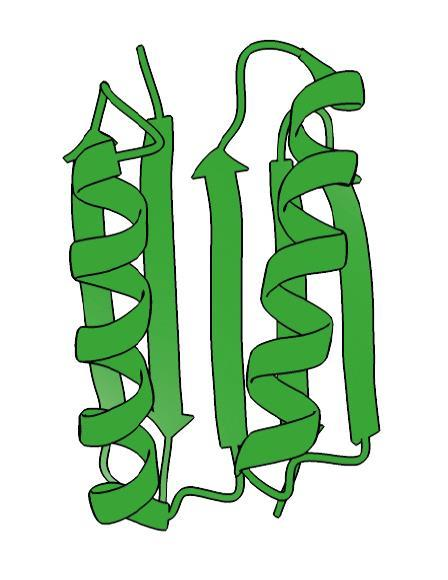
\includegraphics[height=5cm,keepaspectratio]{../../theme/images/protein.png}
        };
      \end{tikzpicture}
      % Title
      \vspace*{0.5cm}
      \begin{center}
        {\Huge\color{iqbblue}\textbf{#2}}\\[0.3cm]
        {\Large\color{iqbgray}#1}
      \end{center}
      \vspace*{0.3cm}
    \endgroup
  \end{frame}
}

\title{New Insights into the Cooperativity and Dynamics of Dimeric Enzymes}
\subtitle{Understanding Why Half of All Enzymes Are Homodimers}
\author{Ke-Wei Chen \and Tian-Yu Sun \and Yun-Dong Wu\textsuperscript{*}}
\institute{%
  深圳湾实验室 化学生物学研究所\\
  北京大学深圳研究生院 化学生物学与生物技术学院\\[0.2cm]
  \textbf{期刊：}\textit{Chemical Reviews} 2023, 123, 9940−9981\\
  \textbf{DOI：}10.1021/acs.chemrev.3c00042%
}
\date{2023年8月10日发表}

% Cover metadata
\papertitlechn{二聚体酶的协同性与动力学}
\papertitlechnsub{一半酶为何以同源二聚体形式存在}
\paperengtitle{New Insights into the Cooperativity and Dynamics of Dimeric Enzymes}

\begin{document}

% ============================================================
% Footer Configuration
% ============================================================
\iqbfootline{default}{title}{pageofy}

% ------------------------------------------------------------
% 1. Cover
% ------------------------------------------------------------
\iqbcoverframe

% ------------------------------------------------------------
% Part 1: Introduction \& Background
% ------------------------------------------------------------
\iqbsectionframe{Introduction}{引言}

% ------------------------------------------------------------
% 2. Why Study Dimeric Enzymes?
% ------------------------------------------------------------
\begin{frame}{超半数酶为同源二聚体：一个不容忽视的生物学现象}
  \iqblayoutcustom[0.40]{
    \iqbsectiontitle{Database统计结果}
    \begin{iqbitemize}
      \item UniProt数据库：各种催化功能的酶，\textbf{同源二聚体}占所有蛋白质结构的\textbf{51\%以上}，远超单体和其他寡聚形式
      \item Brenda数据库：已定义寡聚形式的酶中，\textbf{二聚体数量超过单体}
      \item 偶数亚基($2n$)酶多于奇数亚基($2n-1$)酶
      \item 大多数辅因子依赖酶（NAD, ATP, 金属离子等）以\textbf{同源二聚体}形式存在
    \end{iqbitemize}

  }{
    \iqbfig[height=0.60\textheight]{Figures/Figure01.png}{从19世纪统计力学基础到现代生物分子模拟：同源二聚体酶的演进与普遍性}
  }
\end{frame}

% ------------------------------------------------------------
% 3. Historical Context \& Review Scope
% ------------------------------------------------------------
\begin{frame}{经典理论奠定基础，现代技术揭示机制}
  \iqblayouttwo{
    \iqbsectiontitle{理论基础：协同性概念的建立}
    \begin{iqbitemize}
      \item 1965年：\textbf{Monod-Wyman-Changeux (MWC)模型}为血红蛋白建立\textbf{变构与协同性}理论
      \item Perutz的双结构立体化学模型为理解二聚体酶\textbf{亚基间协同性}提供基础
      \item 亚基间\textbf{变构调节}导致底物/产物亲和力或催化效率差异，通过\textbf{构象变化}实现
    \end{iqbitemize}
  }{
    \iqbsectiontitle{本综述的研究范围}
    \begin{iqbitemize}
      \item 二聚体酶的生物学必要性
      \item 实验和计算研究方法
      \item 底物结合中的协同性
      \item 催化过程中的协同性和动力学机制
      \item 影响催化效率/协同性的关键因素
      \item 亚基界面的重要作用
      \item 二聚体有机催化剂的协同催化
    \end{iqbitemize}
  }
    \iqbsep

    \iqbgreenbox{应用前景}{为设计高效催化剂（如\textbf{二聚体有机催化剂}）和药物（如\textbf{Paxlovid}靶向SARS-CoV-2\textbf{同源二聚体}主蛋白酶）提供理论支撑}
\end{frame}

% ------------------------------------------------------------
% Part 2: Biological Necessity
% ------------------------------------------------------------
\iqbsectionframe{Biological Necessity}{生物学必要性}

% ------------------------------------------------------------
% 4a1. Biological Advantages: Protein Folding
% ------------------------------------------------------------
\begin{frame}{二聚化的生物学优势：促进蛋白质折叠}
  \iqblayouttwo{
    \iqbsectiontitle{促进蛋白质折叠的机制}
    \begin{iqbitemize}
      \item 亚基界面提供额外的\textbf{疏水核心}
      \item 减少\textbf{溶剂暴露表面积}（BSA降低）
      \item 降低\textbf{折叠能量势垒}$\Delta G_{fold}$
      \item 提高折叠效率和成功率
      \item 减少聚集形成包涵体的风险
    \end{iqbitemize}

    \iqbsep

    \iqbsectiontitle{界面形成的热力学驱动}
    \begin{iqbitemize}
      \item \textbf{疏水效应}：疏水残基埋藏释放水分子
      \item \textbf{焓驱动}：界面氢键、盐桥形成
      \item \textbf{熵驱动}：溶剂化水分子释放增加熵
      \item 总自由能：$\Delta G_{bind} = \Delta H - T\Delta S$
    \end{iqbitemize}
  }{
    \iqbsectiontitle{定量数据}
    \begin{iqbitemize}
      \item 典型界面埋藏面积：\textbf{1000-3000 Ų}
      \item 界面自由能：\textbf{-5至-15 kcal/mol}
      \item 解离常数：$K_d$ = \textbf{nM至$\mu$M级别}
      \item BSA减少：\textbf{15-25\%}
    \end{iqbitemize}

    \iqbsep

    \iqbsectiontitle{实例与应用}
    \begin{iqbitemize}
      \item 许多酶的单体形式无法正确折叠
      \item 工业酶工程：通过二聚化提高表达产量
      \item 减少包涵体形成提高可溶性表达
      \item 热休克蛋白辅助二聚化折叠
    \end{iqbitemize}
  }
\end{frame}

% ------------------------------------------------------------

% ------------------------------------------------------------
% 4a2-2. Biological Advantages: Interface Interaction Types
% ------------------------------------------------------------
\begin{frame}{二聚化的生物学优势：界面相互作用网络}
  \iqblayouttwo{
    \iqbsectiontitle{界面相互作用类型}
    \begin{iqbitemize}
      \item 氢键网络：Ser/Thr/Tyr-主链羰基
      \item 盐桥：Arg/Lys-Asp/Glu配对
      \item 疏水相互作用：Leu/Ile/Val/Phe簇
      \item 芳香堆积：Phe/Tyr/Trp $\pi$-$\pi$作用
    \end{iqbitemize}

    \iqbsep

    \iqbsectiontitle{能量贡献}
    \begin{iqbitemize}
      \item 氢键：每个\textbf{2-5 kcal/mol}
      \item 盐桥：每对\textbf{3-7 kcal/mol}
      \item 疏水作用：总\textbf{10-20 kcal/mol}
      \item 芳香堆积：每对\textbf{2-4 kcal/mol}
    \end{iqbitemize}
  }{
    \iqbsectiontitle{工程应用}
    \begin{iqbitemize}
      \item 理性设计增强界面氢键网络
      \item 引入盐桥提升高温稳定性
      \item 优化疏水核心降低解折叠速率
      \item 添加二硫键锁定二聚体构象
      \item 成功案例：嗜热菌酶$T_m$提升至\textbf{95°C}
    \end{iqbitemize}

  \iqbtinysep
    \iqborangebox{工程策略}{\textbf{多重界面相互作用}协同提升\textbf{热稳定性}}
  }
\end{frame}

% ------------------------------------------------------------
% 4b. Biological Advantages: Catalysis & Regulation
% ------------------------------------------------------------
\begin{frame}{二聚化的生物学优势：催化与调控}
  \iqbfontsizemode{small}

  \iqblayouttwo{
    \iqbsectiontitle{3. 催化活性增强}
    \begin{iqbitemize}
      \item 单体通常催化活性极低或无活性
      \item 二聚化诱导\textbf{活性位点形成}或优化
      \item 亚基间\textbf{协同作用}提高$k_{cat}$/降低$K_M$
      \item \textbf{底物通道化}：中间产物直接传递
      \item \textbf{变构调节}：一个亚基影响另一个
      \item 典型案例：HIV蛋白酶、TIM等
    \end{iqbitemize}

    \iqbsep

    \iqbsectiontitle{4. 调控功能实现}
    \begin{iqbitemize}
      \item 单体-二聚体平衡受配体/pH/离子强度调控
      \item Caspase-9等凋亡酶通过\textbf{二聚化激活}
      \item 实现\textbf{开关式调控}：ON/OFF状态
      \item 避免单体在细胞内误触发反应
      \item 提供额外调控层次
    \end{iqbitemize}
  }{
    \iqbsectiontitle{定量效应}
    \begin{iqbitemize}
      \item 催化效率提升：\textbf{2-1000倍}
      \item 底物亲和力提高：$K_M$降低\textbf{10-100倍}
      \item 产物释放加速：$k_{off}$提高
      \item 协同系数：\textbf{Hill系数$n_H > 1$}
    \end{iqbitemize}

    \iqbsep

    \iqbsectiontitle{进化意义}
    \begin{iqbitemize}
      \item 单体→二聚体：功能跃迁
      \item 界面突变扩大功能多样性
      \item 二聚化是蛋白质进化的关键创新
      \item 约35\%的酶是寡聚体
    \end{iqbitemize}

    \iqbsep

    \iqborangebox{核心优势}{二聚化整合\textbf{结构稳定}、\textbf{催化增强}、\textbf{调控精准}}
  }
\end{frame}

% ------------------------------------------------------------
% Part 3: Experimental \& Computational Methods
% ------------------------------------------------------------
\iqbsectionframe{Methods}{实验与计算方法}

% ------------------------------------------------------------
% 5a. MWC Model Mathematical Framework (Figure 2)
% ------------------------------------------------------------
\begin{frame}{MWC模型的数学框架：状态、权重与反应速率}
  \iqbfontsizemode{small}

  \iqblayoutcustom[0.45]{
    \iqbsectiontitle{MWC模型核心假设}
    \begin{iqbitemize}
      \item 酶在\textbf{两种构象状态}间平衡：\textbf{活性态}($E_A$)和\textbf{非活性态}($E_I$)
      \item \textbf{对称性}：二聚体的两个亚基同时处于相同状态
      \item \textbf{预存平衡}：构象转换发生在底物结合之前
      \item 活性态对底物的\textbf{亲和力远高于}非活性态
    \end{iqbitemize}

    \iqbtinysep

    \iqbsectiontitle{状态权重（Boltzmann分布）}
    \begin{iqbitemize}
      \item 活性态：$W_A = e^{-\beta E_A}$
      \item 非活性态：$W_I = e^{-\beta E_I}$
      \item 平衡常数：$L_0 = \frac{[E_I]}{[E_A]} = e^{-\beta(E_I - E_A)}$
      \item $\beta = 1/(k_B T)$，$k_B$为Boltzmann常数
    \end{iqbitemize}
  }{
    \iqbfig[height=0.50\textheight]{Figures/Figure02.png}{MWC模型：状态权重、亲和力和催化速率}
  }
\end{frame}

% ------------------------------------------------------------
% 5b. Protein Dynamics Time Scales (Figure 3)
% ------------------------------------------------------------
\begin{frame}{蛋白质运动的时间尺度：从飞秒到秒}
  \iqbfontsizemode{small}

  \iqblayoutcustom[0.35]{
    \iqbsectiontitle{分子运动的层次结构}
    \begin{iqbitemize}
      \item \textbf{超快运动}(10 fs - 1 ps)：键振动、侧链旋转
      \item \textbf{快速运动}(1 ps - 1 ns)：$\alpha$-螺旋折叠、$\beta$-发夹折叠
      \item \textbf{中等运动}(1 ns - 1 $\mu$s)：Loop运动、二级结构重排
      \item \textbf{慢速运动}(1 $\mu$s - 1 ms)：变构转换、三级结构变化
      \item \textbf{极慢运动}(1 ms - 1 s)：蛋白质折叠、寡聚化
    \end{iqbitemize}

    \iqbtinysep

    \iqbsectiontitle{催化相关时间尺度}
    \begin{iqbitemize}
      \item 底物结合/解离：$\mu$s-ms
      \item 催化反应：ns-$\mu$s
      \item 产物释放：$\mu$s-ms
      \item 变构信号传递：ns-ms
    \end{iqbitemize}
  }{
    \iqbfig[height=0.50\textheight]{Figures/Figure03.png}{蛋白质运动时间尺度：从原子振动到整体折叠}

    \iqbtinysep

    \iqbbluebox{MD挑战}{催化运动跨越\textbf{6-9个数量级}，需\textbf{增强采样}}
  }
\end{frame}

% 4a2-1a. Thermostability: Quantitative Data
% ------------------------------------------------------------
\begin{frame}{二聚化的生物学优势：定量热稳定性数据}
  \iqblayoutcustom[0.35]{
    \iqbsectiontitle{定量数据}
    \begin{iqbitemize}
      \item 二聚体$T_m$比单体高\textbf{10-30°C}
      \item 典型界面埋藏面积：\textbf{1000-3000 Ų}
      \item 每100 Ų界面约提升$T_m$ \textbf{1-2°C}
      \item 解折叠自由能提升\textbf{5-15 kcal/mol}
      \item 蛋白酶解抗性提高\textbf{2-10倍}
    \end{iqbitemize}
  }{
    \iqbfig[height=0.43\textheight]{Figures/Figure04.png}{二聚化稳定构象：亚基界面形成提高酶热稳定性和结构刚性}
  }
\end{frame}

% ------------------------------------------------------------
% 4a2-1b. Thermostability: Stability Mechanism
% ------------------------------------------------------------
\begin{frame}{二聚化的生物学优势：稳定机制}
  \iqblayouttwo{
    \iqbsectiontitle{稳定机制}
    \begin{iqbitemize}
      \item 界面降低展开态构象熵
      \item 氢键盐桥疏水作用协同
      \item 抵抗热变性和蛋白酶解
      \item 界面面积与$\Delta T_m$正相关
    \end{iqbitemize}

    \iqbtinysep

    \iqbsectiontitle{界面相互作用}
    \begin{iqbitemize}
      \item 氢键：\textbf{2-5 kcal/mol}，提供特异性
      \item 盐桥：\textbf{3-7 kcal/mol}，稳定界面
      \item 疏水作用：\textbf{主要驱动力}，占\textbf{60-80\%}
      \item 范德华力：优化界面互补性
    \end{iqbitemize}
  }{
    \iqbsectiontitle{工业应用}
    \begin{iqbitemize}
      \item 嗜热酶工程改造
      \item 提高工业催化剂稳定性
      \item 延长酶制剂保质期
      \item 设计超稳定工业酶
    \end{iqbitemize}

    \iqbtinysep

    \iqbsectiontitle{设计策略}
    \begin{iqbitemize}
      \item 增加界面疏水残基含量
      \item 优化氢键和盐桥网络
      \item 引入二硫键稳定界面
      \item 模拟嗜热菌酶的界面特征
    \end{iqbitemize}
  }
\end{frame}

% ------------------------------------------------------------
% 5c. Allosteric Models in Dimers (Figure 5)
% ------------------------------------------------------------
\begin{frame}{二聚体中的变构模型：MWC、KNF与HT的扩展}
  \iqbfontsizemode{small}

  \iqblayoutcustom[0.35]{
    \iqbsectiontitle{单体到二聚体的模型演化}
    \begin{iqbitemize}
      \item \textbf{单体MWC}：两种构象（T/R），配体选择性结合R态
      \item \textbf{单体KNF}：配体结合诱导构象变化
      \item \textbf{二聚体MWC}：两个亚基对称切换（T$_2$ $\leftrightarrow$ R$_2$）
      \item \textbf{二聚体KNF}：允许非对称中间态（TR、T$_2$S、TRS$_2$等）
      \item \textbf{Hilser-Thompson模型}：考虑固有无序性和折叠/解折叠平衡
    \end{iqbitemize}

    \iqbmicrosep

    \iqbsectiontitle{HT模型的创新之处}
    \begin{iqbitemize}
      \item 蛋白质结构存在局部和全局的无序/有序转换
      \item 配体结合影响整个蛋白质的折叠平衡
      \item 不强调亚基间对称性，更符合实际动力学行为
      \item 熵驱动的变构机制
    \end{iqbitemize}
  }{
    \iqbfig[height=0.40\textheight]{Figures/Figure05.png}{MWC、KNF和HT模型的比较}

    \iqbmicrosep

    \iqbgreenbox{实验验证}{NMR弛豫和FRET动力学实验可精确区分对称与非对称构象态}
  }
\end{frame}

% ------------------------------------------------------------
% 5. Biophysical Experimental Techniques
% ------------------------------------------------------------
\begin{frame}{生物物理实验方法：结构解析与动力学检测}
  \iqblayouttwo{
    \iqbsectiontitle{结构确定技术}
    \begin{iqbitemize}
      \item X射线晶体学：高分辨率静态结构（Å级）
      \item 冷冻电镜（Cryo-EM）：近原子分辨率，适用于大复合物和动态系统
      \item 核磁共振（NMR）：溶液中的动态构象和弛豫时间
      \item 小角X射线散射（SAXS）：溶液态寡聚状态和形状
      \item 质谱（MS）：寡聚状态鉴定、氢氘交换动力学
    \end{iqbitemize}
  }{
    \iqbsectiontitle{酶动力学实验}
    \begin{iqbitemize}
      \item Michaelis-Menten方程：$v = \frac{V_{max}[S]}{K_m + [S]}$
      \item MWC理论：酶在活性（$E_A$）和非活性（$E_I$）状态间切换
      \item 稳态动力学 vs. 预稳态动力学（快速反应）
      \item 同位素示踪、荧光/FRET跟踪构象变化
      \item 等温滴定量热法（ITC）测结合热力学
    \end{iqbitemize}

    \iqbsep

    \iqborangebox{多技术结合}{\textbf{结构+动力学+热力学}的组合实验揭示完整的\textbf{催化机制}}
  }
\end{frame}

% ------------------------------------------------------------
% 6. Computational Simulation Methods
% ------------------------------------------------------------
\begin{frame}{计算模拟方法：从原子到系统层次}
  \iqblayoutthree{
    \iqbsectiontitle{分子动力学模拟}
    \small
    \begin{iqbitemize}
      \item MD：原子级时间演化（ns-$\mu$s尺度）
      \item 增强采样：metadynamics, umbrella sampling, REMD
      \item 机器学习加速：reinforced dynamics (RID)方法
    \end{iqbitemize}

    \iqbtinysep

    \iqbsectiontitle{结合预测}
    \small
    \begin{iqbitemize}
      \item 分子对接：蛋白-配体相互作用
      \item 自由能计算：FEP, TI, MM/GBSA
      \item 打分函数优化
    \end{iqbitemize}
  }{
    \iqbsectiontitle{多尺度模拟}
    \small
    \begin{iqbitemize}
      \item QM/MM：活性位点量子化学+周围MM
      \item 粗粒化模型：长时间尺度和大系统
      \item 网络分析：变构通路预测
    \end{iqbitemize}

    \iqbtinysep

    \iqbsectiontitle{机器学习}
    \small
    \begin{iqbitemize}
      \item 神经网络势能面
      \item 深度学习预测动力学
      \item AlphaFold等结构预测
    \end{iqbitemize}
  }{
    \iqbfig[height=0.45\textheight]{Figures/Figure06.png}{计算方法揭示动态变构网络}
  }
\end{frame}

% ------------------------------------------------------------
% Part 4: Cooperativity in Substrate Binding
% ------------------------------------------------------------
\iqbsectionframe{Substrate Binding}{底物结合中的协同性}

% ------------------------------------------------------------
% 7. Allosteric Models
% ------------------------------------------------------------
\begin{frame}{变构理论：MWC构象选择 vs. KNF诱导契合}
  \iqblayouttwo{
    \iqbsectiontitle{MWC模型（\textbf{Conformational Selection}）}
    \begin{iqbitemize}
      \item 配体\textbf{选择性结合}与底物结合状态相似的主导构象
      \item 强调\textbf{亚基间对称性}维持
      \item 预先存在多种\textbf{离散构象}的平衡
      \item 快速平衡近似：底物结合/解离速率$>$构象转换速率
    \end{iqbitemize}

    \iqbsep

    \iqbsectiontitle{KNF模型（\textbf{Induced Fit}）}
    \small
    \begin{iqbitemize}
      \item 配体随机结合后\textbf{诱导构象转变}至最优态
      \item 允许\textbf{亚基间非对称性}
      \item 第一个配体结合能量影响第二个配体结合
    \end{iqbitemize}
  }{
    \iqbsectiontitle{Hilser-Thompson (HT)模型}
    \begin{iqbitemize}
      \item 蛋白质\textbf{固有无序性}在整个结构中存在
      \item \textbf{折叠与解折叠}的平衡
      \item 配体结合过程中多种构象选择
      \item \textbf{不强调亚基间对称性}
    \end{iqbitemize}

    \iqbsep

    \iqbbluebox{现代观点}{动力学研究表明，\textbf{构象选择（MWC）}可能是配体结合目标蛋白的\textbf{更普遍机制}}
  }
\end{frame}

% ------------------------------------------------------------
% 8. Thermodynamics of Allostery
% ------------------------------------------------------------
\begin{frame}{变构调节的热力学本质：熵与焓的平衡}
  \iqblayoutcustom[0.4]{
    \iqbsectiontitle{超越构象变化的变构}
    \begin{iqbitemize}
      \item 变构不仅是构象改变，更依赖于\textbf{熵和焓}的综合变化
      \item Cooper \& Dryden开创性发现：配体结合改变蛋白质\textbf{热涨落幅度}，而非构象本身
      \item \textbf{"熵驱动"系统}：刚性和柔性区域的再平衡
      \item PKA-C等酶的\textbf{构象熵变化}全局分布于整个酶
    \end{iqbitemize}

    \iqbmicrosep

    \iqbsectiontitle{熵-焓补偿原理}
    \begin{iqbitemize}
      \item $\Delta G = \Delta H - T\Delta S$：\textbf{自由能驱动变构}
      \item 焓变：氢键、盐桥、范德华力的重排
      \item 熵变：构象自由度、溶剂化熵的变化
      \item 温度依赖性：$T\Delta S$项随温度显著变化
    \end{iqbitemize}
  }{
    \iqbfig[height=0.75\textheight]{Figures/Figure07.png}{变构调节：熵-焓补偿原理驱动构象选择与自由能平衡}
  }
\end{frame}

\begin{frame}{变构热力学：动态平衡与实验测量}
  \iqblayouttwo{
    \iqbsectiontitle{动态平衡与涨落}
    \begin{iqbitemize}
      \item 蛋白质构象系综的热涨落
      \item 配体结合重塑能量景观
      \item 亚基间动态耦合传递熵变
      \item 构象选择vs诱导契合机制
    \end{iqbitemize}

    \iqbmicrosep

    \iqbsectiontitle{温度效应}
    \begin{iqbitemize}
      \item 温度升高增强构象涨落
      \item 熵-焓补偿维持$\Delta G$稳定
      \item 变构效应的温度敏感性
    \end{iqbitemize}
  }{
    \iqbsectiontitle{实验测量}
    \begin{iqbitemize}
      \item ITC（等温滴定量热）：直接测$\Delta H$
      \item van't Hoff分析：温度依赖性获取$\Delta S$
      \item NMR弛豫：构象熵的动力学信息
      \item MD模拟：熵贡献的计算分解
    \end{iqbitemize}

    \iqbmicrosep

    \iqbsectiontitle{二聚体特性}
    \begin{iqbitemize}
      \item 亚基间熵变耦合
      \item 界面形成的熵焓平衡
      \item 协同性的热力学基础
    \end{iqbitemize}
  }
\end{frame}

% ------------------------------------------------------------
% Part 5: Cooperativity in Catalysis
% ------------------------------------------------------------
\iqbsectionframe{Catalysis}{催化过程中的协同性}

% ------------------------------------------------------------
% 9. Half-of-the-Sites Reactivity
% ------------------------------------------------------------
\begin{frame}{半位点反应性：为何只有一个亚基催化？}
  \iqblayoutcustom[0.37]{
    \iqbsectiontitle{半位点反应性}
    \begin{iqbitemize}
      \item 二聚体中\textbf{只有一个位点}结合并催化底物
      \item 另一亚基无法结合或结合但\textbf{不催化}
      \item 广泛存在于碱性磷酸酶、脱卤酶等
    \end{iqbitemize}

    \iqbtinysep

    \iqbsectiontitle{协同性类型}
    \begin{iqbitemize}
      \item \textbf{正协同性}：提高催化效率
      \item \textbf{负协同性}：降低酶活性
      \item 非催化亚基可促进或抑制催化
    \end{iqbitemize}

    \iqbtinysep

    \iqbgreenbox{关键概念}{\textbf{底物结合亲和力}变化不等同于\textbf{催化效率}提升，需区分\textbf{结合协同性}与\textbf{催化协同性}}
  }{
    \iqbfig[height=0.58\textheight]{Figures/Figure08.png}{半位点反应性的分子基础：亚基间构象不对称性}
  }
\end{frame}

% ------------------------------------------------------------
% 10. Negative Cooperativity Mechanisms
% ------------------------------------------------------------
\begin{frame}{负协同性的四种分子机制}
  \iqblayouttwo{
    \iqbsectiontitle{Koshland 1971年提出的四种模型}
    \begin{enumerate}
      \item 异源二聚体：两个单体具有不同催化活性，形成结构和功能不对称的异二聚体
      \item 同源二聚体形变：亚基相同但不对称结合时一个位点变形失去结合能力
      \item 空间位阻：二聚化后两个底物结合口袋过于接近，第一个底物阻碍第二个底物结合
      \item 变构诱导：配体结合产生构象变化，改变空亚基使其无法结合底物
    \end{enumerate}
  }{
    \iqbsectiontitle{现代理解：变构整体模型}
    \begin{iqbitemize}
      \item 单纯基于结合口袋的模型无法完全捕捉同源二聚化产生的构象运动
      \item 变构整体模型：酶蛋白构象变化复杂且全局，对维持催化位点最优活性必不可少
      \item 可能在调控蛋白(如激活/抑制蛋白)或核受体蛋白中更为普遍
    \end{iqbitemize}

    \iqbsep

    \iqborangebox{生物学意义}{\textbf{负协同性}确保\textbf{底物识别特异性}，避免非特异性催化}
  }
\end{frame}

% ------------------------------------------------------------
% 11. Positive Cooperativity: Three Mechanisms
% ------------------------------------------------------------
\begin{frame}{正协同性的三种关键生物学特性}
  \iqbfontsizemode{small}

  \iqblayoutcustom[0.4]{
    \iqbsectiontitle{1. 空亚基动力学}
    \begin{iqbitemize}
      \item 一个亚基结合配体，另一个保持空置
      \item 空亚基通过"熵增"参与催化
      \item FAcD案例：空亚基释放水分子、构象涨落增大
      \item 提供热力学驱动力
    \end{iqbitemize}

    \iqbtinysep

    \iqbsectiontitle{2. 催化效率提升}
    \begin{iqbitemize}
      \item 非催化亚基通过变构调节增强催化
      \item 底物通道形成、静电优化
      \item 质子/电子传递通路建立
      \item 热容减少(MMRT理论)
    \end{iqbitemize}

    \iqbtinysep

    \iqbsectiontitle{3. 底物-产物耦合}
    \begin{iqbitemize}
      \item 交替催化位点模型
      \item 亚基A产物释放与亚基B底物结合耦合
      \item 缩短催化周期时间
    \end{iqbitemize}
  }{
    \iqbfig[height=0.52\textheight]{Figures/Figure09.png}{正协同性三大机制：底物诱导、构象选择与动态变构}

    \iqbmicrosep

    \iqbgreenbox{协同效应}{空亚基动力学、催化效率提升和底物产物耦合三大机制协同作用显著提高催化效率}
  }
\end{frame}

% ------------------------------------------------------------
% 10-11. Interface Network and Drug Design Preview
% ------------------------------------------------------------

% ------------------------------------------------------------
% 14b1-1a. Interface: Transmission Mechanism
% ------------------------------------------------------------
\begin{frame}{过渡态理论与抑制剂设计：TSID策略}
  \iqbfig[height=0.35\textheight]{Figures/Figure10.png}{过渡态理论与TSID (Transition State Inhibitor Design)：底物→过渡态→产物}
  \iqbtinysep

  \iqblayouttwo{
    \iqbsectiontitle{过渡态理论}
    \begin{iqbitemize}
      \item 过渡态比底物更稳定结合
      \item 酶活性位点互补过渡态
      \item 降低反应能垒关键机制
      \item 决定酶催化效率
    \end{iqbitemize}
  }{
    \iqbsectiontitle{TSID抑制剂设计}
    \begin{iqbitemize}
      \item 模拟过渡态结构特征
      \item 比底物结合更高效
      \item 创造高效抑制剂策略
      \item 二聚体酶抑制剂开发基础
    \end{iqbitemize}
  }
\end{frame}

\begin{frame}{仿生催化剂设计启示：从酶学习什么？}
  \iqblayouttwo{
    \iqbsectiontitle{二聚体酶的核心优势}
    \begin{iqbitemize}
      \item 双位点协同：底物通道、静电场、质子/电子传递
      \item 动态变构网络：蛋白质骨架传递远程信号
      \item 熵驱动机制：空亚基动力学补偿
      \item 精细调控：通过界面调节寡聚状态和活性
    \end{iqbitemize}

    \iqbsep

    \iqbsectiontitle{小分子催化剂的局限}
    \begin{iqbitemize}
      \item 缺乏大规模构象变化能力
      \item 难以实现远程变构传递
      \item 协同机制主要依赖空间接近效应
    \end{iqbitemize}
  }{
    \iqbsectiontitle{设计策略}
    \begin{iqbitemize}
      \item 引入柔性连接臂模拟蛋白质骨架
      \item 利用超分子自组装构建动态催化体系
      \item 金属-有机框架(MOF)中固定双位点
      \item 计算辅助设计：预测协同效应
      \item 定向进化：筛选最优连接臂长度和角度
    \end{iqbitemize}

    \iqbsep

    \iqbbluebox{终极目标}{创造兼具酶的高效协同性和小分子催化剂广泛底物谱的新型催化系统}
  }
\end{frame}

% ------------------------------------------------------------
% 16. Drug Design: Paxlovid Example
% ------------------------------------------------------------
\begin{frame}{药物设计实例：靶向SARS-CoV-2主蛋白酶的Paxlovid}
  \iqbfontsizemode{small}

  \iqblayoutcustom[0.4]{
    \iqbsectiontitle{SARS-CoV-2主蛋白酶(M$^{\text{pro}}$)}
    \begin{iqbitemize}
      \item 同源二聚体形式
      \item 病毒复制必需酶，切割多蛋白前体
      \item 催化二元：Cys145- His41组成半胱天冬氨酸样活性位点
      \item 二聚化对催化活性至关重要
      \item 单体几乎无活性
    \end{iqbitemize}

    \iqbtinysep

    \iqbsectiontitle{Paxlovid (Nirmatrelvir)设计策略}
    \small
    \begin{iqbitemize}
      \item 共价抑制剂，与Cys145形成可逆共价键
      \item 结合二聚体活性位点与S1/S2袋的构象特征
      \item 通过理解二聚体界面驱动的协同机制优化药效
      \item 高选择性、强效、口服生物利用度高
    \end{iqbitemize}
  }{
    \iqbfig[height=0.66\textheight]{Figures/Figure11.png}{Paxlovid结合M$^{\text{pro}}$二聚体活性位点的分子机制}
  }
\end{frame}

% ------------------------------------------------------------
% 12. Positive Cooperativity Properties (Figure 12)
% ------------------------------------------------------------
\begin{frame}{正协同性的生物物理特征：实验表征与理论预测}
  \iqbfontsizemode{small}

  \iqblayoutcustom[0.35]{
    \iqbsectiontitle{Hill系数与协同性强度}
    \begin{iqbitemize}
      \item \textbf{Hill系数$n_H$}：衡量协同性的\textbf{定量指标}
      \item \textbf{$n_H > 1$：正协同性}；\textbf{$n_H < 1$：负协同性}；$n_H = 1$：无协同性
      \item 理论最大值：$n_H = n$(亚基数)，二聚体最大为\textbf{2}
      \item 实际测量值通常小于理论值，反映部分协同
    \end{iqbitemize}

    \iqbmicrosep

    \iqbsectiontitle{动力学表现}
    \begin{iqbitemize}
      \item \textbf{S型（sigmoid）}底物浓度-反应速率曲线
      \item 陡峭的响应曲线：生理调控优势
      \item \textbf{$K_{0.5}$}：达到半最大速率的底物浓度
      \item 可通过突变或辅因子改变协同性强度
    \end{iqbitemize}
  }{
    \iqbfig[height=0.5\textheight]{Figures/Figure12.png}{正协同性的Hill曲线特征：$n_H$、$K_{0.5}$与S型动力学响应}

  \iqbmicrosep
    \iqborangebox{生物学意义}{正协同性\textbf{Hill系数大于1}使酶快速响应浓度变化实现\textbf{代谢开关调控}}
  }
\end{frame}

% ------------------------------------------------------------
% 13. Empty Subunit Dynamics: FAcD Case (Figure 13)
% ------------------------------------------------------------
\begin{frame}{空亚基动力学：脱卤酶FAcD的熵驱动协同性}
  \iqblayoutcustom[0.40]{
    \iqbsectiontitle{FAcD酶的空亚基现象}
    \begin{iqbitemize}
      \item 脱卤酶（FAcD）：催化卤代脂肪酸脱卤
      \item 实验观察：一个亚基结合底物时，另一个亚基保持空置
      \item 空亚基并非惰性旁观者，而是主动参与催化
      \item MD模拟揭示空亚基经历显著构象涨落
    \end{iqbitemize}

    \iqbtinysep

    \iqbsectiontitle{熵补偿机制}
    \begin{iqbitemize}
      \item 底物结合导致催化亚基熵减（$\Delta S < 0$）
      \item 空亚基通过增大构象涨落提供熵增（$\Delta S > 0$）
      \item 释放界面水分子进一步增加体系熵
      \item 总自由能变化：$\Delta G = \Delta H - T\Delta S_{total}$更负，反应更有利
    \end{iqbitemize}
  }{
    \iqbfig[height=0.55\textheight]{Figures/Figure13.png}{FAcD空亚基：熵增补偿底物结合熵减}

    \iqbtinysep

  }
\end{frame}

% ------------------------------------------------------------
% 14. Catalytic Cooperativity: SaMTAN Case (Figure 14)
% ------------------------------------------------------------
\begin{frame}{催化协同性实例：SaMTAN的双重调控机制}
  \iqbfontsizemode{small}

  \iqblayoutcustom[0.38]{
    \iqbsectiontitle{SaMTAN酶简介}
    \begin{iqbitemize}
      \item 5\textquotesingle-甲硫腺苷/ S-腺苷同型半胱氨酸核糖苷酶（MTAN）
      \item 水解MTA/SAH的N-糖苷键，生成腺嘌呤与5-thioribosyl基
      \item 同源二聚体结构，每个亚基含独立催化位点
      \item 第一催化位点亲和力高（约0.1\,$\mu$M），$n_H \approx 1.8$
    \end{iqbitemize}

    \iqbsep

    \iqbsectiontitle{亚基间通讯路径}
    \begin{iqbitemize}
      \item 单个位点占据时催化速率较慢
      \item 底物占据第二位点需等待第一位点产物释放
      \item 界面氢键网络存储应变能，促进相邻亚基产物释放
      \item 关键残基突变可将协同性降为$\;n_H \rightarrow 1$
    \end{iqbitemize}
  }{
    \iqbfig[height=0.6\textheight]{Figures/Figure14.png}{SaMTAN氢键网络介导正协同性：界面残基传递构象变化提升催化}
  }
\end{frame}

% ------------------------------------------------------------
% 15. Subunit Functional Asymmetry: ADAR2 Case (Figure 15)
% ------------------------------------------------------------
\begin{frame}{亚基功能不对称：ADAR2的结构-功能分工}
  \iqbfontsizemode{small}

  \iqblayoutcustom[0.38]{
    \iqbsectiontitle{ADAR2的RNA编辑功能}
    \begin{iqbitemize}
      \item 双链RNA特异的腺苷脱氨酶：将A转为I
      \item 每条链包含C端脱氨酶结构域与多个dsRBD
      \item 晶体结构显示同源二聚体呈功能不对称
      \item 一条链主导催化，另一条链通过dsRBD负责RNA识别/定位
    \end{iqbitemize}

    \iqbtinysep

    \iqbsectiontitle{不对称性的分子基础}
    \begin{iqbitemize}
      \item 二聚界面结合RNA形成蛋白-蛋白/蛋白-RNA复合
      \item dsRBD2靠近RNA双链，帮助定位目标序列
      \item 另一个亚基的脱氨酶结构域直接承担催化
      \item 功能分工提升整体编辑效率与特异性
    \end{iqbitemize}
  }{
    \iqbfig[height=0.42\textheight]{Figures/Figure15.png}{ADAR2二聚体的功能不对称：催化与识别动态交替}

    \iqbtinysep

  }
\end{frame}

% ------------------------------------------------------------
% 16. Substrate Channel: HisFH Case (Figure 16)
% ------------------------------------------------------------
\begin{frame}{底物通道化实例：组氨酸生物合成酶HisFH}
  \iqbfontsizemode{small}

  \iqblayoutcustom[0.4]{
    \iqbsectiontitle{HisFH的双功能催化}
    \begin{iqbitemize}
      \item HisH亚基水解谷氨酰胺生成谷氨酸与NH$_3$
      \item NH$_3$沿约25Å通道传递到HisF亚基
      \item HisF将输送来的NH$_3$与底物PrFAR反应
      \item 生成组氨酸前体ImGP与AICAR，实现跨亚基协作
    \end{iqbitemize}

    \iqbtinysep

    \iqbsectiontitle{底物通道的结构与功能}
    \begin{iqbitemize}
      \item 亚基间形成封闭隧道，限制NH$_3$和中间体逸散
      \item 疏水环境稳定反应中间体并指导其方向
      \item 通道出口残基对ImGP前体精准定位
      \item 通道化避免扩散损失并提高总体催化效率
    \end{iqbitemize}
  }{
    \iqbfig[height=0.50\textheight]{Figures/Figure16.png}{HisFH底物通道：PRFAR在20Å封闭通道内亚基间直接传递}

    \iqbtinysep

  }
\end{frame}

% ------------------------------------------------------------
% 17. Substrate Channel: JMJD1A Case (Figure 17)
% ------------------------------------------------------------
\begin{frame}{去甲基化酶JMJD1A：底物通道机制}
  \iqbfig[height=0.28\textheight]{Figures/Figure17.png}{JMJD1A底物通道：me1中间产物在亚基间传递}
  \iqbmicrosep

  \iqblayoutcustom[0.40]{
    \iqbsectiontitle{JMJD1A的组蛋白去甲基化功能}
    \begin{iqbitemize}
      \item Jumonji C (JmjC)家族Fe(II)/$\alpha$-酮戊二酸依赖酶
      \item 选择性去除H3K9的单甲基与二甲基（me1/me2）
      \item 同源二聚体：两个活性位点彼此协作
      \item 每步反应伴随产生甲醛与琥珀酸
    \end{iqbitemize}

    \iqbmicrosep

  }{
    \iqbsectiontitle{底物通道的独特优势}
    \begin{iqbitemize}
      \item me2在一亚基被转化为me1后沿通道传递至另一亚基
      \item 避免未完全去甲基化的组蛋白提前释放
      \item 保持H3K9修饰正确重塑，防止异常染色质状态
      \item 任何活性位点突变都会显著削弱两步催化
    \end{iqbitemize}
  }
\end{frame}

% ------------------------------------------------------------
% 18. Electrostatic Environment Modulation (Figure 18)
% ------------------------------------------------------------
\begin{frame}{静电环境调控：亚基通过静电场协同优化催化}
  \iqbfontsizemode{small}

  \iqblayoutcustom[0.38]{
    \iqbsectiontitle{静电场对催化的影响}
    \begin{iqbitemize}
      \item 酶活性位点的局部静电场影响反应势垒
      \item 带电残基、金属离子、偶极形成复杂电场分布
      \item 一个亚基的构象变化改变相邻亚基的静电环境
      \item 协同优化过渡态稳定化
    \end{iqbitemize}

    \iqbmicrosep

    \iqbsectiontitle{实验与计算证据}
    \begin{iqbitemize}
      \item 界面带电残基突变显著影响$k_{cat}$(催化速率常数)
      \item QM/MM计算揭示亚基间静电相互作用
      \item 底物结合后，空亚基的偶极重排优化催化亚基电场
      \item 典型案例：碱性磷酸酶、核酸酶等
    \end{iqbitemize}
  }{
    \iqbfig[height=0.48\textheight]{Figures/Figure18.png}{亚基间静电相互作用调控电场}

  }
\end{frame}

% ------------------------------------------------------------
% 19. Proton Wire Communication (Figure 19)
% ------------------------------------------------------------
\begin{frame}{质子线通讯：亚基间质子传递网络}
  \iqblayoutcustom[0.35]{
    \iqbsectiontitle{质子线的概念与结构}
    \begin{iqbitemize}
      \item 由连续氢键网络形成的质子传递通路
      \item 涉及氨基酸侧链、骨架羰基、水分子
      \item 格罗图斯机制：质子快速接力传递
      \item 亚基质子化状态影响相邻亚基催化活性
    \end{iqbitemize}

    \iqbtinysep

    \iqbsectiontitle{质子耦合的催化协同}
    \begin{iqbitemize}
      \item 一个亚基催化反应产生的质子
      \item 通过质子线传递至另一个亚基
      \item 激活第二个催化位点或促进产物释放
      \item 实例：脱氢酶、氧化还原酶等
    \end{iqbitemize}
  }{
    \iqbfig[height=0.58\textheight]{Figures/Figure19.png}{质子线网络：氢键链介导质子传递与协同}

    \iqbtinysep

  }
\end{frame}

% ------------------------------------------------------------
% 20. Electron Transfer: Cytochrome bc1 Case (Figure 20)
% ------------------------------------------------------------
\begin{frame}{电子传递协同：细胞色素bc$_1$复合物}
  \iqbfontsizemode{small}

  \iqblayoutcustom[0.42]{
    \iqbsectiontitle{Cytbc$_1$的电子传递链}
    \begin{iqbitemize}
      \item 线粒体呼吸链复合物III
      \item 二聚体结构，每个单体含多个氧化还原中心
      \item 催化醌的氧化和细胞色素c的还原
      \item Q循环机制：2个电子分别传递至不同亚基
    \end{iqbitemize}

    \iqbmicrosep

    \iqbsectiontitle{亚基间电子协同}
    \begin{iqbitemize}
      \item 一个亚基的电子传递影响另一亚基的氧化还原电位
      \item 铁硫簇（ISP）在两个亚基间摆动传递电子
      \item 协同确保电子传递方向性和防止副反应（超氧生成）
      \item 二聚体界面调控ISP的构象动力学
    \end{iqbitemize}

    \iqbmicrosep
    \iqborangebox{能量转换}{电子传递耦合质子泵送}
  }{
    \iqbfig[height=0.69\textheight]{Figures/Figure20.png}{Cytbc$_1$二聚体的电子传递协同：ISP摆动实现跨亚基电子传递}
  }
\end{frame}

% ------------------------------------------------------------
% 21a. Negative Heat Capacity: Theoretical Basis
% ------------------------------------------------------------
\begin{frame}{负热容机制I：Makhatadze-Privalov理论基础}
  \iqbfontsizemode{small}

  \iqblayoutcustom[0.45]{
    \iqbsectiontitle{热容与蛋白质动力学}
    \begin{iqbitemize}
      \item 热容$C_p = (\partial H / \partial T)_p$：能量涨落的度量
      \item 蛋白质折叠/结合通常伴随$\Delta C_p < 0$
      \item Makhatadze-Privalov模型：负$\Delta C_p$源于疏水效应
      \item 底物结合减少溶剂可及表面积（SASA）
    \end{iqbitemize}

    \iqbtinysep

    \iqbsectiontitle{热容变化的分子起源}
    \begin{iqbitemize}
      \item 疏水残基埋藏释放溶剂化水分子
      \item 水分子从有序界面层转为自由bulk水
      \item 减少系统能量涨落幅度
      \item SASA减少与$\Delta C_p$呈线性关系
    \end{iqbitemize}
  }{
    \iqbsectiontitle{定量关系}
    \begin{iqbitemize}
      \item $\Delta C_p \approx -0.32$ cal/(mol·K·Å²) × $\Delta$SASA
      \item 蛋白质折叠：$\Delta C_p$ = -1至-3 kcal/(mol·K)
      \item 底物结合：$\Delta C_p$ = -0.1至-0.5 kcal/(mol·K)
      \item 负$\Delta C_p$使结合焓与温度相关
    \end{iqbitemize}

    \iqbtinysep

    \iqbsectiontitle{实验测定方法}
    \begin{iqbitemize}
      \item ITC：等温滴定量热法直接测$\Delta H(T)$
      \item DSC：差示扫描量热法测$C_p(T)$曲线
      \item Van't Hoff分析：温度依赖的平衡常数
    \end{iqbitemize}
  }
\end{frame}

% ------------------------------------------------------------
% 21b-1a. Negative Heat Capacity: Heat Capacity Change
% ------------------------------------------------------------
\begin{frame}{负热容机制：底物结合的热容变化}
  \iqblayoutcustom[0.32]{
    \iqbsectiontitle{热容变化}
    \begin{iqbitemize}
      \item 亚基结合底物后界面疏水残基暴露减少
      \item 导致整个二聚体的热容降低
      \item 典型$\Delta C_p$值：-1 to -3 kcal/(mol·K)
      \item 影响相邻亚基构象涨落和结合亲和力
    \end{iqbitemize}

    \iqbtinysep

    \iqbsectiontitle{协同效应}
    \begin{iqbitemize}
      \item 负热容反映二聚体协同性强度
      \item 热容变化与Hill系数正相关
      \item 界面疏水作用主导热容效应
      \item 温度敏感性源于水化熵变化
    \end{iqbitemize}
  }{
    \iqbfig[height=0.45\textheight]{Figures/Figure21.png}{负热容效应：疏水残基埋藏导致$\Delta C_p < 0$}

    \iqbtinysep

    \iqbsectiontitle{实验测量}
    \begin{iqbitemize}
      \item ITC测量热焓，DSC测定热容
      \item 范特霍夫分析验证$\Delta C_p$
    \end{iqbitemize}
  }
\end{frame}

% ------------------------------------------------------------
% 21b-1b. Negative Heat Capacity: Mechanism & Compensation (MERGED)
% ------------------------------------------------------------
\begin{frame}{负热容机制：分子机制与熵-焓补偿}
  \iqblayouttwo{
    \iqbsectiontitle{分子机制}
    \begin{iqbitemize}
      \item 疏水残基去水合减少水分子自由度
      \item 界面紧密接触降低构象熵
      \item 水分子从界面释放到溶液
      \item 整体热容降低反映有序度提高
    \end{iqbitemize}

    \iqbmicrosep

    \iqbsectiontitle{定量关系}
    \begin{iqbitemize}
      \item $\Delta C_p \propto$ 疏水表面积变化
      \item 每100 Ų界面约-0.2 kcal/(mol·K)
      \item 负$\Delta C_p$越大协同性越强
    \end{iqbitemize}
  }{
    \iqbsectiontitle{熵-焓补偿机制}
    \begin{iqbitemize}
      \item 负热容是熵-焓补偿的热力学基础
      \item 温度升高：$\Delta H$和$\Delta S$同时变化
      \item 两者抵消保持$\Delta G$相对稳定
      \item 使酶在宽温度范围内保持活性
    \end{iqbitemize}

    \iqbmicrosep

    \iqbsectiontitle{生物学意义}
    \begin{iqbitemize}
      \item 适应不同温度环境
      \item 保持催化效率稳定性
      \item 提高酶的环境适应性
    \end{iqbitemize}
  }
\end{frame}

% ------------------------------------------------------------
% 21c. Negative Heat Capacity in Dimeric Enzymes - Part 2
% ------------------------------------------------------------
\begin{frame}{负热容机制：空亚基的热容贡献}
  \iqblayouttwo{
    \iqbsectiontitle{非催化亚基的热容贡献}
    \begin{iqbitemize}
      \item 非催化亚基对负$\Delta C_p$有显著贡献
      \item 贡献区域远离活性中心，分布于整个蛋白
      \item 空亚基贡献可达总$\Delta C_p$的30-50\%
      \item 通过界面传递影响催化亚基的动力学
    \end{iqbitemize}

    \iqbtinysep

    \iqbsectiontitle{二聚体vs单体的热容效应}
    \begin{iqbitemize}
      \item 单体酶的远端结构域贡献无法与二聚体相比
      \item 二聚化创造了新的协同热容调控机制
      \item 分布式热容效应增强催化稳定性
      \item 一个亚基的热容变化影响另一亚基的构象分布
      \item 实现协同性与催化效率的热力学耦合
    \end{iqbitemize}
  }{
    \iqbsectiontitle{生物学意义}
    \begin{iqbitemize}
      \item 使二聚体酶适应温度波动环境
      \item 提高催化反应的温度适应性
      \item 在进化上选择二聚体构型的热力学优势
      \item 为酶工程设计提供热稳定性改造策略
    \end{iqbitemize}
  }

  \iqbtinysep

  {\tiny\iqborangebox{协同效应}{空亚基通过热容贡献影响催化亚基动力学}}
\end{frame}

% ------------------------------------------------------------
% 22. Heat Capacity Differences in Cooperativity (Figure 22)
% ------------------------------------------------------------
\begin{frame}{热容差异与协同性：MMRT理论应用}
  \iqbfontsizemode{small}

  \iqblayoutcustom[0.36]{
    \iqbsectiontitle{MMRT理论（Macromolecular Rate Theory）}
    \begin{iqbitemize}
      \item Hobbs等提出的酶催化速率温度依赖性理论
      \item 核心假设：$\Delta C_p^{\ddagger} \neq 0$（活化热容不为零）
      \item 解释非Arrhenius行为：曲线型Eyring plot
      \item $k_{cat}(T) = \frac{k_B T}{h} e^{-\Delta G^{\ddagger}(T)/RT}$
    \end{iqbitemize}

    \iqbtinysep

    \iqbsectiontitle{二聚体酶的热容协同}
    \begin{iqbitemize}
      \item 一个亚基结合底物后，降低过渡态的$C_p^{\ddagger}$
      \item 减少热涨落，稳定过渡态构象
      \item 相邻亚基通过界面感知热容变化
      \item 调整自身构象以匹配最优催化温度
    \end{iqbitemize}
  }{
    \iqbfig[height=0.50\textheight]{Figures/Figure22.png}{MMRT理论：温度依赖性协同通过热容变化调控催化效率}
  }
\end{frame}

% ------------------------------------------------------------
% 23. Substrate/Product Coupling (Figure 23)
% ------------------------------------------------------------
\begin{frame}{底物结合-产物释放耦合：交替位点催化模型}
  \iqblayoutcustom[0.36]{
    \iqbsectiontitle{交替催化位点机制}
    \begin{iqbitemize}
      \item 一个亚基催化反应并释放产物
      \item 同时触发另一个亚基结合新底物
      \item 两个亚基交替进行底物结合和产物释放
      \item 类似"跷跷板"效应：一侧产物离去，另一侧底物进入
    \end{iqbitemize}

    \iqbmicrosep

    \iqbsectiontitle{热力学与动力学耦合}
    \begin{iqbitemize}
      \item 产物释放的$\Delta G$驱动构象变化
      \item 该构象变化提高相邻亚基对底物的亲和力
      \item 缩短总催化周期时间：$\tau_{total} < \tau_{uncoupled}$
      \item 实验证据：单分子FRET、快速动力学
    \end{iqbitemize}
  }{
    \iqbfig[height=0.45\textheight]{Figures/Figure23.png}{底物-产物耦合机制：一个亚基底物结合促进另一亚基产物释放}

    \iqbmicrosep

    \iqbgreenbox{催化效率倍增}{亚基间底物结合与产物释放的耦合显著缩短催化周期时间，催化效率远超单体加和}
  }
\end{frame}

% ------------------------------------------------------------
% 24. F-ATPase Rotational Catalysis (Figure 24)
% ------------------------------------------------------------
\begin{frame}{F-ATPase旋转催化：协同性的终极体现}
  \iqbimgcenter[height=0.42\textheight]{Figures/Figure24.png}

  \iqblayouttwo{
    \iqbsectiontitle{Boyer结合变化机制}
    \begin{iqbitemize}
      \item 三个$\beta$亚基循环经历三种构象：O(open), L(loose), T(tight)
      \item 旋转$\gamma$亚基驱动构象切换
      \item T态：ATP合成；L态：ADP+Pi结合；O态：ATP释放
      \item 每120°旋转，三个亚基同步切换构象
    \end{iqbitemize}
  }{
    \iqbsectiontitle{质子驱动与机械耦合}
    \begin{iqbitemize}
      \item F$_0$亚基的质子流驱动$\gamma$亚基旋转
      \item 旋转力矩通过$\gamma$轴传递至$\beta$亚基
      \item 机械能转化为化学能（ATP合成）
      \item 效率>90\%，接近热力学极限
    \end{iqbitemize}
  }
\end{frame}

% ------------------------------------------------------------
% Part 6: Factors Affecting Cooperativity
% ------------------------------------------------------------
\iqbsectionframe{Influencing Factors}{影响协同性的因素}

% ------------------------------------------------------------
% 13. Key Factors 
% ------------------------------------------------------------
\begin{frame}{影响催化效率与协同性的关键因素}
  \iqblayouttwo{
    \iqbsectiontitle{辅因子/配体或pH诱导的构象/寡聚形式变化}
    \begin{iqbitemize}
      \item 金属离子（Mg$^{2+}$, Zn$^{2+}$）诱导单体-二聚体转换
      \item pH依赖性：质子化状态改变影响界面相互作用
      \item NAD/NADP等辅因子结合稳定二聚体
      \item 变构效应物调节活性构象分布
    \end{iqbitemize}

    \iqbsep

    \iqbsectiontitle{突变或氨基酸修饰导致的环境变化}
    \begin{iqbitemize}
      \item 界面残基突变改变单体-二聚体平衡
      \item 磷酸化、乙酰化等翻译后修饰调控寡聚状态
      \item 疏水核心突变影响热稳定性
    \end{iqbitemize}
  }{
    \iqbsectiontitle{同源酶之间的差异}
    \begin{iqbitemize}
      \item 不同物种的同源酶底物结合协同性可能相反
      \item 例：大肠杆菌D-乳酸脱氢酶显示正协同性，而铜绿假单胞菌同源酶显示负协同性
      \item 反映酶的物种特异性和对催化环境的高度依赖
    \end{iqbitemize}

    \iqbsep

    \iqbsectiontitle{界面水分子}
    \small
    \begin{iqbitemize}
      \item 亚基界面水分子对调节协同性极为重要
      \item FAcD中观察到沿反应坐标周期性变化的界面水分子
      \item 血红蛋白含氧/脱氧态分别含11和17个界面水分子
      \item 调节蛋白活动性和配体逃逸
    \end{iqbitemize}
  }
\end{frame}

% ------------------------------------------------------------
% Part 7: The Subunit-Subunit Interface
% ------------------------------------------------------------
\iqbsectionframe{Interface}{亚基界面的作用}

% ------------------------------------------------------------
% 25a. Interface Structure (Figure 25 part 1)
% ------------------------------------------------------------
\begin{frame}{亚基界面的结构功能：稳定性基础}
  \iqbfontsizemode{small}

  \iqblayoutcustom[0.30]{
    \iqbsectiontitle{结构特征}
    \begin{iqbitemize}
      \item 疏水核心+氢键网络+盐桥
      \item 埋藏面积：1000-3000 Ų
      \item BSA与$\Delta G$线性相关
      \item 残基高度保守
      \item 互补表面形状匹配
    \end{iqbitemize}

    \iqbmicrosep

    \iqbsectiontitle{界面分类}
    \begin{iqbitemize}
      \item 永久界面：刚性紧密堆积
      \item 瞬态界面：动态可逆装配
      \item 调控界面：响应信号变化
      \item 混合型：兼具多种特性
    \end{iqbitemize}

    \iqbmicrosep

    \iqbsectiontitle{功能整合}
    \begin{iqbitemize}
      \item 结构支撑：稳定二聚体构象
      \item 信号传递：变构通讯通路
      \item 动态调控：响应配体结合
    \end{iqbitemize}
  }{
    \iqbfig[height=0.75\textheight]{Figures/Figure25.png}{界面的三重功能：结构支撑、信号传递、动态调控}
  }
\end{frame}

% ------------------------------------------------------------
% 25b. Interface Communication & Regulation
% ------------------------------------------------------------
\begin{frame}{亚基界面的通讯与调控功能}
  \iqblayouttwo{
    \iqbsectiontitle{通讯功能}
    \begin{iqbitemize}
      \item 变构通路连接活性位点
      \item 关键残基：高betweenness centrality
      \item 动态网络揭示信息流
      \item 界面突变切断/重定向通讯
    \end{iqbitemize}

    \iqbtinysep

    \iqbsectiontitle{调控功能}
    \begin{iqbitemize}
      \item 寡聚化平衡调控
      \item pH/离子强度敏感
      \item 翻译后修饰调节
      \item 配体诱导界面重排
    \end{iqbitemize}
  }{
    \iqbsectiontitle{设计应用}
    \begin{iqbitemize}
      \item 蛋白质工程：改造界面
      \item 药物设计：靶向二聚化
      \item 变构调节剂开发
      \item 人工酶界面设计
    \end{iqbitemize}

  \iqborangebox{设计启示}{理解界面是调控二聚化和协同性的关键}
  }
\end{frame}

% ------------------------------------------------------------
% 14a. Interface Importance: Long-range Allosteric Interaction
% ------------------------------------------------------------
\begin{frame}{亚基界面：残基网络与长程变构传递}
  \iqblayoutcustom[0.35]{
    \iqbsectiontitle{界面残基网络作用}
    \begin{iqbitemize}
      \item 界面残基网络传递变构信号至活性位点
      \item 残基形成连续相互作用链
      \item 关键残基作为信号传递节点
      \item 变构通路长度通常10-25 Å
    \end{iqbitemize}

    \iqbsep

    \iqbsectiontitle{界面热点残基}
    \begin{iqbitemize}
      \item 热点残基在界面高度聚集
      \item 单个残基突变可显著改变$K_d$和$k_{cat}$
      \item 界面扰动远距离影响活性位点
      \item 通常为保守的疏水或带电残基
    \end{iqbitemize}
  }{
    \iqbfig[height=0.70\textheight]{Figures/Figure25.png}{界面长程相互作用与位点间通讯}
  }
\end{frame}

\begin{frame}{亚基界面：路径优化与实验证据}
  \iqblayouttwo{
    \iqbsectiontitle{路径优化机制}
    \begin{iqbitemize}
      \item 多条冗余路径提高鲁棒性
      \item 瓶颈残基控制传递强度
      \item 进化选择最优网络拓扑
      \item 路径长度与效率的平衡
    \end{iqbitemize}

    \iqbsep

    \iqbsectiontitle{定量分析}
    \begin{iqbitemize}
      \item 界面突变影响催化效率达2-3个数量级
      \item 界面水分子网络参与信号传递
      \item 变构路径涉及10-20个关键残基
    \end{iqbitemize}
  }{
    \iqbsectiontitle{实验证据}
    \begin{iqbitemize}
      \item MD模拟揭示变构通路和动态网络
      \item 双突变循环分析揭示残基耦合
      \item 时间分辨晶体学捕获传递瞬态
      \item 进化耦合分析预测关键接触
    \end{iqbitemize}

    \iqbsep

    \iqbsectiontitle{工程应用}
    \begin{iqbitemize}
      \item 指导理性突变设计
      \item 优化酶工程改造策略
      \item 药物靶点识别
    \end{iqbitemize}
  }
\end{frame}

% ------------------------------------------------------------
% 14b1-1b. Interface: Dynamic Features + Experimental Validation (MERGED)
% ------------------------------------------------------------
\begin{frame}{亚基界面：构象传递的动力学特征与实验验证}
  \iqbfontsizemode{small}

  \iqblayouttwo{
    \iqbsectiontitle{动力学特征}
    \begin{iqbitemize}
      \item 快速相：ns级局部调整
      \item 慢速相：$\mu$s-ms整体构象变化
      \item 多时间尺度协同耦合
      \item 能垒高度决定传播速率
    \end{iqbitemize}

    \iqbmicrosep

    \iqbsectiontitle{实验技术}
    \begin{iqbitemize}
      \item NMR弛豫：捕获构象变化动力学
      \item FRET：测量亚基间距离变化
      \item MD模拟：揭示变构通路
      \item 突变分析：鉴定关键传递残基
    \end{iqbitemize}

    \iqbmicrosep

    \iqbsectiontitle{关键发现}
    \begin{iqbitemize}
      \item 构象变化时间尺度：$\mu$s-ms
      \item 亚基间距离变化：2-5 Å
      \item 变构路径涉及10-20个关键残基
      \item 突变单个残基Hill系数从2降至1
    \end{iqbitemize}
  }{
    \iqbsectiontitle{速率控制机制}
    \begin{iqbitemize}
      \item 局部残基重排控制快速相
      \item 整体构象变化限制慢速相
      \item 温度影响构象涨落幅度
    \end{iqbitemize}

    \iqbmicrosep

    \iqbsectiontitle{生物学意义}
    \begin{iqbitemize}
      \item 快速响应底物结合信号
      \item 精确控制催化周转速率
      \item 多时间尺度保证高效协同
      \item 动态平衡维持酶活性
    \end{iqbitemize}

    \iqbmicrosep

    \iqbsectiontitle{工程应用启示}
    \begin{iqbitemize}
      \item 界面残基网络是协同性结构基础
      \item 变构路径精确调控保证催化效率
      \item 残基保守性反映功能重要性
      \item 为酶工程设计提供分子机制
    \end{iqbitemize}
  }
\end{frame}


% ------------------------------------------------------------
% 14b1-2a. Interface: Network Properties + Experimental Validation (MERGED)
% ------------------------------------------------------------
\begin{frame}{亚基界面：残基网络特性与实验验证}
  \iqblayouttwo{
    \iqbsectiontitle{网络特性}
    \begin{iqbitemize}
      \item 残基间距离<5 Å形成紧密接触
      \item 氢键和范德华力维持网络稳定性
      \item 保守残基在进化中高度保守
      \item 突变单个关键残基可完全破坏协同性
    \end{iqbitemize}

    \iqbmicrosep

    \iqbsectiontitle{实验证据}
    \begin{iqbitemize}
      \item 双突变循环分析揭示残基耦合
      \item 进化耦合分析预测关键接触
      \item 结构比对显示网络保守性
      \item 分子动力学模拟验证传递路径
    \end{iqbitemize}
  }{
    \iqbsectiontitle{功能意义}
    \begin{iqbitemize}
      \item 网络完整性决定协同效应强度
      \item 关键节点残基控制信号传递
      \item 冗余路径保证功能鲁棒性
      \item 进化优化网络拓扑结构
    \end{iqbitemize}

    \iqbmicrosep

    \iqbsectiontitle{技术应用}
    \begin{iqbitemize}
      \item 预测未知残基相互作用
      \item 指导理性突变设计
      \item 优化酶工程改造策略
      \item 网络分析指导药物靶点设计
    \end{iqbitemize}
  }
\end{frame}

% ------------------------------------------------------------
% 14b2. Interface: Proton Transmission
% ------------------------------------------------------------
\begin{frame}{亚基界面：质子传递机制}
  \iqbfontsizemode{small}

  \iqblayouttwo{
    \iqbsectiontitle{质子传递特征}
    \begin{iqbitemize}
      \item 界面氢键网络或质子线传递
      \item 传播速率：ns级别，远快于构象变化
      \item His/Glu/Asp等可质子化残基
      \item 界面水分子参与质子传递链
    \end{iqbitemize}

    \iqbtinysep

    \iqbsectiontitle{动力学优势}
    \begin{iqbitemize}
      \item 质子传递比构象变化快3-6个数量级
      \item 保证催化效率不受构象重排限制
      \item 实现亚基间快速信号传递
    \end{iqbitemize}
  }{
    \iqbsectiontitle{生物学意义}
    \begin{iqbitemize}
      \item 加速催化循环周转
      \item 提高酶的催化效率
      \item 精确控制反应时序
    \end{iqbitemize}

    \iqborangebox{协同效应}{质子传递速率保证催化协同性}
  }
\end{frame}

% ------------------------------------------------------------
% 14b. Interface Importance: Communication Mechanisms Part 2
% ------------------------------------------------------------
\begin{frame}{亚基界面：电子与静电场传递机制}
  \iqbfontsizemode{small}

  \iqblayouttwo{
    \iqbsectiontitle{电子传递机制}
    \begin{iqbitemize}
      \item 氧化还原酶通过界面金属簇传递电子
      \item 传递距离：可达10-15 Å跨越界面
      \item 涉及Fe-S簇、血红素等辅因子
      \item 电子隧穿效率随距离指数衰减
    \end{iqbitemize}

    \iqbtinysep

    \iqbsectiontitle{静电场传递机制}
    \begin{iqbitemize}
      \item 带电残基重排改变局部静电势
      \item 作用范围：15-20 Å远程影响
      \item 调控底物结合和过渡态稳定
      \item 一个亚基的电场变化影响另一亚基催化
    \end{iqbitemize}
  }{
    \iqbsectiontitle{协同效应}
    \begin{iqbitemize}
      \item 四种机制通常协同作用
      \item 不同机制时间尺度互补
      \item 保证亚基间信息精确传递
      \item 实现高效协同催化
    \end{iqbitemize}

    \iqbtinysep

  }
\end{frame}

% ------------------------------------------------------------
% 14b. Interface Importance: Water Network Dynamics
% ------------------------------------------------------------
\begin{frame}{亚基界面：水分子网络的动态作用}
  \iqbfontsizemode{small}

  \iqblayouttwo{
    \iqbsectiontitle{界面水网络的功能}
    \begin{iqbitemize}
      \item 响应构象变化：水网络结构重组传递信号
      \item 质子传递介质：形成质子线（proton wire）
      \item 熵驱动补偿：空亚基界面水分子释放增加熵
      \item 稳定过渡态：界面水网络稳定催化过渡态
    \end{iqbitemize}

    \iqbtinysep

    \iqbsectiontitle{水分子的热力学贡献}
    \begin{iqbitemize}
      \item 界面埋藏释放10-20个水分子
      \item 每个水分子释放贡献熵：$\sim$+5 cal/(mol·K)
      \item 总熵变：$\Delta S \sim$ +50至+100 cal/(mol·K)
      \item 自由能贡献：$-T\Delta S \sim$ -15至-30 kcal/mol
    \end{iqbitemize}
  }{
    \iqbsectiontitle{实验证据}
    \begin{iqbitemize}
      \item 中子衍射：直接观测界面水分子位置
      \item MD模拟：揭示水网络动态重组过程
      \item 氘代实验：测定质子传递路径
      \item ITC：测定水释放的熵-焓补偿
    \end{iqbitemize}

    \iqbtinysep

  }
\end{frame}

% ------------------------------------------------------------
% 14b. Interface Importance: Evolutionary Significance
% ------------------------------------------------------------
\begin{frame}{亚基界面：进化创新的枢纽}
  \iqblayouttwo{
    \iqbsectiontitle{促进酶进化}
    \begin{iqbitemize}
      \item 界面突变改变寡聚状态：单体$\leftrightarrow$二聚体$\leftrightarrow$多聚体
      \item 二聚化扩大进化搜索空间
      \item 单体→二聚体：功能跃迁的关键步骤
      \item 界面氨基酸进化速率通常高于活性位点
    \end{iqbitemize}

    \iqbtinysep

    \iqbsectiontitle{进化优势的定量分析}
    \begin{iqbitemize}
      \item 二聚体酶约占所有酶的35\%
      \item 界面面积与功能复杂度正相关
      \item 通过界面工程可快速获得新功能
      \item 天然二聚体的界面通常高度保守
    \end{iqbitemize}

    \iqbtinysep

    \iqbbluebox{核心作用}{界面是协同性与酶进化的分子枢纽}
  }{
    \iqbsectiontitle{界面作为药物靶点}
    \begin{iqbitemize}
      \item 靶向界面可破坏二聚化，消除活性
      \item 与活性位点相比，界面更易于选择性抑制
      \item 实例：HIV蛋白酶二聚化抑制剂
      \item 界面小分子调节剂可实现变构调控
    \end{iqbitemize}

    \iqbtinysep

    \iqbsectiontitle{工程应用前景}
    \begin{iqbitemize}
      \item 通过界面设计创造新型催化活性
      \item 调节界面亲和力优化酶活性
      \item 人工二聚化系统：化学诱导二聚化（CID）
      \item 合成生物学中的多酶复合物设计
    \end{iqbitemize}
  }
\end{frame}

% ------------------------------------------------------------
% Part 8: Implications \& Applications
% ------------------------------------------------------------
\iqbsectionframe{Applications}{应用前景}

% ------------------------------------------------------------
% 26. Dimeric Organic Catalysts (Figure 26)
% ------------------------------------------------------------
\begin{frame}{二聚体有机催化剂：酶协同性的仿生应用}
  \iqbfontsizemode{small}

  \iqblayoutcustom[0.4]{
    \iqbsectiontitle{仿生设计原理}
    \begin{iqbitemize}
      \item 模拟二聚体酶的双催化位点架构
      \item 手性配体二聚：如Trost配体、BINOL衍生物
      \item 协同效应：双位点同时作用于底物不同部位
      \item 立体选择性增强：ee值从单体的50-70\%提升至>95\%
    \end{iqbitemize}

    \iqbtinysep

    \iqbsectiontitle{典型案例}
    \begin{iqbitemize}
      \item 双手性膦配体：不对称氢化反应
      \item 双Lewis酸催化剂：Diels-Alder反应
      \item 双质子供体/受体催化剂：Michael加成
      \item 相比单体，反应速率提高2-20倍
    \end{iqbitemize}
    \iqbtinysep

    \iqborangebox{设计挑战}{需引入柔性连接臂实现构象协同}
  }{
    \iqbfig[height=0.7\textheight]{Figures/Figure26.png}{二聚体有机催化剂：双位点协同}

  }
\end{frame}

% ------------------------------------------------------------
% 27. Binuclear Metal Catalysts (Figure 27)
% ------------------------------------------------------------
\begin{frame}{双核金属催化剂：金属协同的仿酶催化}
  \iqbfontsizemode{small}

  \iqblayoutcustom[0.36]{
    \iqbsectiontitle{双核金属中心的协同机制}
    \begin{iqbitemize}
      \item 模拟金属酶：酪氨酸酶（Cu-Cu）、甲烷单加氧酶（Fe-Fe）
      \item 双金属间电子传递：混合价态稳定化
      \item 协同底物活化：一个金属结合底物，另一个活化氧化剂
      \item 桥联配体调控金属间距和电子耦合
    \end{iqbitemize}

    \iqbtinysep

    \iqbsectiontitle{实例与应用}
    \begin{iqbitemize}
      \item Co-salen二聚体：CO$_2$/环氧化物共聚合
      \item Ru-Ru双核配合物：水氧化催化（人工光合作用）
      \item Pd-Pd双核催化剂：C-H活化与偶联反应
      \item TOF(转化频率)提高10-100倍
    \end{iqbitemize}
  }{
    \iqbfig[height=0.50\textheight]{Figures/Figure27.png}{双核金属催化剂的协同催化}

    \iqbtinysep

  }
\end{frame}

% ------------------------------------------------------------
% Summary: Biocatalyst Design Insights
% ------------------------------------------------------------

% ------------------------------------------------------------
% Part 9: Conclusions \& Future Directions
% ------------------------------------------------------------
\iqbsectionframe{Conclusions}{总结与展望}

% ------------------------------------------------------------
% 17. Summary
% ------------------------------------------------------------
\begin{frame}{总结：二聚体酶协同性研究的核心要点}
  \iqbbluebox{关键发现}{
    \begin{iqbitemize}
      \item 超过50\%的酶以同源二聚体形式存在，具有重要生物学意义
      \item 二聚化提供折叠、稳定性、活性和调控四重优势
      \item MWC、KNF、HT模型揭示底物结合中的变构与协同性
      \item 负协同性确保底物识别特异性，正协同性提升催化效率
      \item 正协同性三大机制：空亚基动力学、催化增强、底物结合耦合产物释放
      \item 亚基界面是协同性和进化的枢纽
      \item 辅因子、pH、突变、界面水分子等因素调控协同性
      \item 为设计仿生催化剂和靶向二聚体酶的药物提供理论基础
    \end{iqbitemize}
  }
\end{frame}

% ------------------------------------------------------------
% 18. Future Directions
% ------------------------------------------------------------
\begin{frame}{未来研究方向与挑战}
  \iqblayouttwo{
    \iqbsectiontitle{基础研究}
    \begin{iqbitemize}
      \item 深度学习在酶催化机制预测中的应用
      \item AlphaFold等结构预测工具结合动力学模拟
      \item 单分子技术实时观测亚基间协同动力学
      \item 构象熵和焓的精确量化
      \item 界面水分子动力学的高分辨率研究
    \end{iqbitemize}

    \iqbtinysep

    \iqbsectiontitle{应用研究}
    \small
    \begin{iqbitemize}
      \item 理性设计具有构象变化能力的二聚体有机催化剂
      \item 双核金属催化剂的协同机制优化
      \item 靶向二聚体酶界面的变构抑制剂开发
      \item 工业酶的热稳定性和活性改造
    \end{iqbitemize}
  }{
    \iqbsectiontitle{新兴方向}
    \begin{iqbitemize}
      \item 机器学习预测界面热点残基和变构通路
      \item 从头设计人工二聚体酶
      \item 多酶复合物中的协同性网络
      \item 非平衡态热力学在酶催化中的应用
      \item 膜蛋白二聚体（如受体、转运蛋白）的协同性研究
    \end{iqbitemize}

    \iqbtinysep

    \iqborangebox{跨学科机遇}{结合结构生物学、计算化学、生物信息学和深度学习，全面理解并利用二聚体酶的协同催化}
  }
\end{frame}

% ------------------------------------------------------------
% 19. Acknowledgment \& References
% ------------------------------------------------------------
\begin{frame}{致谢与参考文献}
  \iqbsectiontitle{原文信息}
  \begin{iqbitemize}
    \item \textbf{标题：}New Insights into the Cooperativity and Dynamics of Dimeric Enzymes
    \item \textbf{作者：}Ke-Wei Chen, Tian-Yu Sun, Yun-Dong Wu*
    \item \textbf{期刊：}Chemical Reviews 2023, 123, 9940−9981
    \item \textbf{DOI：}10.1021/acs.chemrev.3c00042
    \item \textbf{发表日期：}2023年8月10日
    \item \textbf{通讯作者：}吴云东 教授 (深圳湾实验室、北京大学深圳研究生院)
  \end{iqbitemize}

  \iqbsep

  \iqbgreenbox{综述的贡献}{系统总结了二聚体酶协同性和动力学的最新研究进展，为酶催化机制研究和催化剂设计提供了全面的理论框架}

\end{frame}

\end{document}
